\newpage
\usecasebase{Accesso alla prenotazione}
\label{usecase:Accesso alla prenotazione}

\begin{figure}[h]
	\centering
	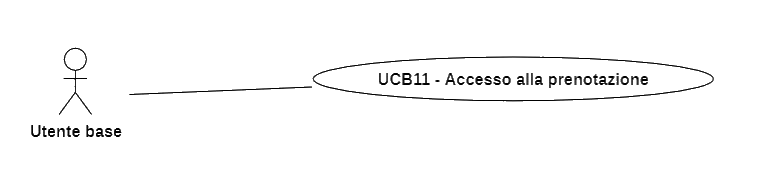
\includegraphics[width=0.8\textwidth]{./uml/UCB11.png} 
	\caption{Accesso alla prenotazione}
	\label{fig:UCB11}
  \end{figure}

\begin{itemize}
	\item \textbf{Attore principale:} Utente base.

	\item \textbf{Precondizioni:} 
	\begin{itemize}
		\item L'Utente base ha effettuato l'accesso al Sistema (vedi \autoref{usecase:Effettua accesso}).
		\item L'Utente base ha ricevuto il \textit{link} di invito ad una prenotazione (vedi \autoref{usecase:Condivisione della prenotazione}).
	\end{itemize}
		

	\item \textbf{Postcondizione:} L'Utente base è collegato ad una prenotazione.

	\item \textbf{Scenario principale:}
	      \begin{enumerate}
		      \item L'Utente base ha ricevuto il \textit{link} di invito ad una prenotazione da parte di un altro utente;
		      \item L'Utente base accetta l'invito;
		      \item L'Utente base è ora collegato ad una prenotazione.
	      \end{enumerate}
\end{itemize}
